\begin{figure}
\centering
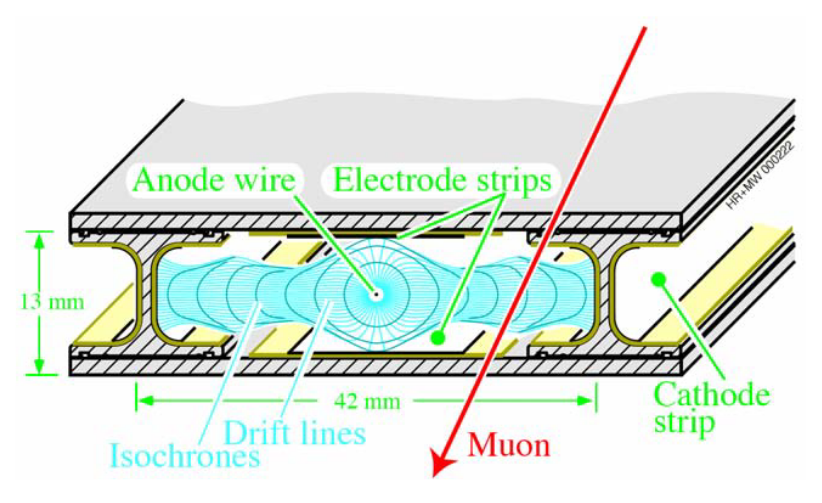
\includegraphics[width=0.7\textwidth]{figures/lhc_and_cms/drift_cell}
\caption{Sketch of a CMS muon system drift cell showing drift lines and isochrones.  The plates at the top and bottom of the cell are at ground potential while the voltages applied to the electrodes are +\SI{+3600}{\V} for wires, +\SI{1800}{\V} for strips, and \SI{-1200}{\V} for cathodes~\cite{cms_experiment}.}
\label{drift_cell}
\end{figure}